\documentclass[titlepage]{article}

\usepackage[utf8]{inputenc}
\usepackage[english]{babel} 
\usepackage{lineno, a4wide} % add line numbers
\linenumbers
\usepackage{setspace} % to use double spacing
\doublespacing

\usepackage{authblk} % author and affiliations
\usepackage{amssymb, amsmath} % for math formulas
\usepackage{amsfonts} % blackboard math symbols
\usepackage[round]{natbib} % citation format
\usepackage{hyperref} % creates links in the document
\usepackage{doi} % Create correct hyperlinks for DOI numbers
\usepackage{times} %Select Adobe Times Roman (or equivalent) as default font

\usepackage{graphicx} % handling figures
\usepackage{subfig} % handling figures
\usepackage[nofiglist,figuresonly]{endfloat} % figures in the end
%\usepackage[nomarkers,figuresonly]{endfloat}
\usepackage{enumitem} % Control layout of itemize, enumerate, description
\usepackage{xcolor} % colored fonts

\usepackage[colorinlistoftodos]{todonotes} % to do comments

\usepackage{subfiles}
\usepackage{parskip}
\usepackage{multirow}
\usepackage[para,online,flushleft]{threeparttable}
\usepackage{rotating}
\usepackage{tikz}
\usepackage{tcolorbox}
\usepackage[export]{adjustbox}[2011/08/13]

\title{
Estimating the cumulative impacts and the zone of influence from multiple anthropogenic infrastructure on biodiversity  \\
{\normalsize in preparation for \textit{Journal of Applied Ecology}}
}

% authors
\author[1,2,*]{Bernardo Brandão Niebuhr}
\author[1,*]{Bram Van Moorter} 
\author[1]{Manuela Panzacchi}
\author[3]{Torkild Tveera}
\author[3]{Knut Langeland}
\author[4]{Audun Stien}
\author[1]{Olav Strand}
\author[5]{Per Sandström}
\author[2]{Anna Skarin}
\author[6]{Moudud Alam}

% affiliation
\affil[1]{Norwegian Institute for Nature Research (NINA), Trondheim, Norway}
\affil[2]{Swedish University of Agricultural Sciences (SLU), Uppsala, Sweden}
\affil[3]{Norwegian Institute for Nature Research (NINA), Tromsø, Norway}
\affil[4]{University of Tromsø, Tromsø, Norway}
\affil[5]{Swedish University of Agricultural Sciences (SLU), Umeå, Sweden}
\affil[6]{Dalarna University, Falun, Sweden}
\affil[*]{Joint first coautorship}
%\affil[+]{Corresponding author: Bernardo Brandão Niebuhr, Norwegian Institute for Nature Research (NINA), Trondheim, Norway; bernardo.brandao@nina.no, bernardo\_brandaum@yahoo.com.br}

\date{Corresponding author: Bernardo Brandão Niebuhr \\Norwegian Institute for Nature Research, Trondheim, Norway \\Contact: bernardo.brandao@nina.no, bernardo\_brandaum@yahoo.com.br \\ Word count: 7850 \\ \today}

\begin{document}

\maketitle

\begin{abstract}

\begin{enumerate}

    \item Most infrastructure and land use change from industrial development take place in landscapes already affected by multiple human disturbances, leading to cumulative impacts on biodiversity. Typically, the effect of infrastructure is determined by computing the distance to the nearest feature only, ignoring their potential to sum up.
    %, mostly because we lack a comprehensive framework to quantify cumulative impacts. 
    Here we propose an approach to estimate the magnitude and the zone of influence (ZoI) of the impacts of multiple features of a given type of infrastructure and test if they accumulate.
    
    \item First, we derive the estimation methods based on the influence from the nearest feature only and the cumulative influence of multiple features.
    Second, we perform simulations to investigate under which conditions these two measures of influence represent different gradients of spatial variation.
    %, and how the area affected by the infrastructure change as the impacts of each of them accumulate. 
    We show the two measures are more correlated either when the spatial distribution of features is sparse and the ZoI is small 
    %(when the minimum distance between features is smaller than the ZoI) 
    or when features are clustered and ZoI is large. 
    %(the ZoI is larger than the size of clusters of features).
    
    \item Finally, we illustrate this approach by assessing the cumulative impacts of tourism facilities on the space use of mountain reindeer, a species highly sensible to anthropogenic activity and infrastructure. We present strong evidence of cumulative impacts of private cottages and tourist cabins on reindeer habitat selection, with zones of influence of 10 and 20 km, respectively. This means that considering only the influence of the nearest feature, as it is common in applied studies, disregards the possibility of cumulative impacts and might limit our understanding of the impacts of landscape change on biodiversity.
    
    %\item To make this approach widely accessible for ecologists and analysts dealing with development, wildlife management, and biodiversity conservation, we also provide tools to allow the quantification of cumulative impacts in both R and GRASS GIS through the \verb|oneimpact| R package.
    
    \item \textit{Synthesis and applications}. We developed an approach to assess cumulative impacts of infrastructure on biodiversity and ecosystems, with direct application in environmental and strategic impact assessment and integrated land use planning. The two influence measures are calculated before statistical analysis, making them computationally efficient and flexible in terms of the choice of influence shape within the ZoI. Both of them can be easily computed in R and GRASS GIS through the \verb|oneimpact| R package. Even though our examples focus on animal space use, the approach can be easily extended to ecological studies and impact assessments over several fields, from genetics to organisms to populations and communities.
\end{enumerate}

\keywords{\textbf{Key-words:} (choose up to 8) cumulative effects, piece-meal development, Anthropocene, habitat fragmentation, habitat loss, \textit{Rangifer tarandus}, density, nearest neighbor distance, scale of effect, kernel filter, distance-weighting}

\end{abstract}

\section{Introduction}

Human-induced land cover modifications and infrastructure from industrial development are widespread and increasing at an accelerated pace across all regions of the world \citep{venter_sixteen_2016,ibisch_global_2016}, including all global biodiversity hotspots \citep{sloan_remaining_2014}, and are among the main causes of biodiversity declines \citep{benitez-lopez_impacts_2010,newbold_global_2015}. Most new landscape changes take place not in intact habitats but in landscapes already affected by multiple disturbances to wildlife \citep{barber_roads_2014}. As a consequence, the effects of such new modifications might accumulate and interact in complex ways with the preexisting anthropogenic stressors, leading to cumulative impacts \citep[Box 1; ][]{gillingham_integration_2016} -- synergistic, interactive, or unpredictable outcomes, different from those of each separate source of disturbance \citep{naugle_unifying_2011}. 
%This process is tackled in the discussion about ``nibbling" and ``piece-meal development" \citep{nellemann_progressive_2003} and have been addressed under the name of cumulative anthropogenic impacts \citep[Box 1; ][]{gillingham_integration_2016}. 
Indeed, cumulative impacts are a central issue in ecological studies and environmental impact assessments and a priority for making effective, knowledge-based decisions on land use planning, designing mitigation actions, and avoiding higher impacts of industrial development on ecosystems \citep{gillingham_integration_2016, laurance_roads_2017}. Most environmental impact assessment studies still focus on single projects at small spatiotemporal scales \citep{johnson_regulating_2011}, and even ecological studies conducted at larger extents generally consider only the effect the nearest feature of each infrastructure type \citep[e.g.][]{torres_assessing_2016}. Here we propose an approach to assess the impacts of multiple features of a given type of infrastructure on biodiversity and test if they accumulate. 

%There have been increasing efforts to better define, review, and outline approaches for cumulative impact assessment \citep{naugle_unifying_2011,gillingham_integration_2016}, yet we still lack a comprehensive framework to quantify cumulative impacts and thus concretely help sustainable land use planning.

Anthropogenic infrastructure have direct consequences in the area where they are built (e.g. habitat modification or road kills), but might also indirectly affect species and ecological processes up to several kilometers from the infrastructure locations \citep[e.g. reducing the probability of animal occurrence][]{johnson_cumulative_2005,torres_assessing_2016}. Therefore, two intrinsically related dimensions of impacts to be assessed in impact studies are the magnitude of the impact and the size of the affected area \citep[Box 1; ][]{naugle_unifying_2011}. The \textit{effect size} or \textit{magnitude of the impact} represents how strongly different factors influence focal organisms and processes and is generally estimated through a combination of biological and environmental data and statistical modeling \citep[Box 1;][]{polfus_identifying_2011}. The spatiotemporal \textit{zone of influence} (ZoI) 
%is intrinsically related to the magnitude of the impacts and 
corresponds to the area (and sometimes the period) within which there are detectable impacts from different landscape modifications on the process of interest, but is commonly expressed in terms of distances --- the distance from or radius around the disturbance sources which defines the affected area \citep[Box 1;][]{ boulanger_estimating_2012}. 

Infrastructure and disturbance impacts can accumulate over time and space, as a result of the sum or interaction of the impacts of different types of infrastructure or multiple features of same-type infrastructure. 
%The consequences of multiple types of infrastructure are generally included in ecological models by careful evaluation of their correlations \citep{dormann_collinearity_2013} and subsequently through the inclusion of additive or interactive terms in statistical model specification, to control for their mutual potential influence on the studied system [REF]. This allows one to estimate the coefficients that represent the magnitude of the impact for each infrastructure or their combination. Alternatively, other studies combine multiple disturbances in a single measure of cumulative effect before fitting statistical models \citep{venter_sixteen_2016, tucker_moving_2018}. 
The cumulative influence of multiple infrastructure of the same type -- our focus here -- is most commonly either appraised by changing the variable's level of spatial organization (e.g. urban areas or wind parks instead of a combination of buildings and turbines, respectively) or ignored by considering only the effect of the nearest infrastructure feature \citep[e.g.][]{torres_assessing_2016}. When determining the ZoI, the concept of ecological threshold %\citep{huggett_concept_2005} 
and analytical procedures developed therein are commonly used \citep{ficetola_ecological_2009}. Under this framework, the estimation of the ZoI is often carried out by fitting piece-wise regression or other non-linear regression models \citep[such as an exponential decay or generalized additive models;][]{skarin_out_2018, ficetola_ecological_2009} to the measured response of an ecosystem as a function of distance to an infrastructure. This distance is typically the distance to the nearest instance of this infrastructure type, ignoring potential cumulative effects of multiple instances of an infrastructure. Besides, this approach is generally limited to the assessment of thresholds for only one or a few types of infrastructure \citep[e.g.][]{boulanger_estimating_2012}, since its computation requires repeated fitting and might become impracticable for a large number of factors \citep{lee_estimating_2020}. 

Another approach to estimate the ZoI may be found under the umbrella of the discussion about spatial and temporal \textit{scales of effect} in the evaluation of species-landscape relationships. In this context, the number of features is averaged for multiple spatial extents surrounding focal study sites \citep{jackson_are_2015} or considering different grains \citep{laforge_process-focussed_2015}, or weighted using neighborhood analysis over several different extents or radii (generally termed ``scales"), creating a series of infrastructure density maps \citep{mcgarigal_multi-scale_2016}. These spatial extents and grains are generally linked to the spatial and temporal dimensions of the infrastructure considered, as well as to the expected temporal scale of the biological response to such infrastructure. Each of these maps is tested against the ecological response variables to assess the extent at which the impact is stronger, most commonly through measures of model performance and explanatory power such as R\textsuperscript{2}, AIC, or BIC, or evaluating the variation in fitted model coefficients \citep{jackson_are_2015, huais_multifit_2018} -- what is called a multi-scale approach \citep[e.g.][]{zeller_multi-level_2017}.
%, in contrast to single-scale analyses in which the effect of all variables is evaluated with the same extent.
Multi-scale analyses brought important advances for landscape and environmental impact studies \citep[e.g.][]{mcgarigal_multi-scale_2016}, even though in many of them the scale of effect was not properly evaluated \citep{jackson_are_2015}. However, the key here is that these approaches have hardly been put into the framework of cumulative impact assessment \citep[but see][]{polfus_identifying_2011}.

We propose an approach to estimate the magnitude and the ZoI of the impacts of multiple features of an infrastructure and test if they accumulate. First, we derive the estimation methods based on either the influence from the nearest feature only or the cumulative influence of multiple features (Box 1, Fig. \ref{fig:zoi_conceptual}), using habitat selection analyses as example. Second, we perform simulations to distinguish in which conditions these two measures of influence represent similar or different spatial gradients, to aid the interpretation of estimated impacts based on each of them. 
Finally, we illustrate our approach by assessing the cumulative effects on the space use of the tundra's flagship species, the mountain reindeer (\textit{Rangifer tarandus tarandus}). We also provide tools to allow an easy implementation of the cumulative approach presented here in R \citep{r_core_team_r_2020} and GRASS GIS \citep{grass_development_team_geographic_2017} through the \verb|oneimpact| R package.

\begin{tcolorbox}[width=1.3\textwidth,center,colback=yellow!5,colframe=yellow!75!black,title={Box 1 -- Definitions}]

\begin{description}

    \item[Impact] The term is used here to represent the consequences of human-made and industrial landscape changes on a focal ecological response variable, such as measures of biodiversity or ecological processes. Thus, impacts represent the functional responses of species and processes to human activity \citep{naugle_unifying_2011}. We analytically decompose the impacts into their \textbf{magnitude} and \textbf{zone of influence (ZoI)}. A given infrastructure (e.g. tourist cabin) might affect a certain process (e.g. an species occurrence) strongly or weakly (magnitude), and this impact might decrease fast with distance or extend over several kilometers (ZoI).
    
    \item[Cumulative impacts] can result from the interaction between multiple features of an infrastructure -- our focus here -- but also from the effects of different types infrastructure (e.g. houses, turbines, roads, dams) or from top-down or bottom-up ecological cascades. Cumulative impacts of multiple features depend on the number of features in an area, their spatial distribution, and co-occurrence with other infrastructure types, and might differ for distinct species, values, or processes -- possibly leading to stronger negative impacts for some or even to benefits for others, if compared to the impact of a single infrastructure.
    
    \item[Magnitude of the impact] It describes how strong is the effect of a variable over a given biological response, and is described here by the model coefficients ($\beta$'s in eq. \ref{eqn:HSF}). 
    
    \item[Influence] The term is used here in a pragmatic way and represents the function $\phi$ that sets how the impacts of an infrastructure feature change with the distance to such feature, and is the basis for defining the ZoI. The influence of a feature might follow different \textbf{influence functions} (also called weighting functions, smoothing filters, or decay functions). It can be constant up to a given threshold distance or decrease in different ways with increasing distance from it (Fig. \ref{fig:zoi_conceptual}A). When multiple features of an infrastructure are present, one can assume that either only the nearest feature affect the response (eq. \ref{eqn:HSFnearest}) or that the influence of multiple features accumulate (eq. \ref{eqn:HSFcuminf}, Fig. \ref{fig:zoi_conceptual}B).
    
    \item[Zone of Influence] The \textbf{ZoI} is the maximum distance from an infrastructure feature where it influences or affects a given biological response. For non-vanishing functions (e.g. exponential, Gaussian), a threshold must be set to define the ZoI -- e.g. the distance at which the influence function goes below 0.05 or 0.01. 
    %Here we call this threshold $\phi_{limit}$.
    In the landscape ecology literature the ZoI is often called the \textit{scale of effect} of a given covariate in space \citep[e.g.][]{jackson_are_2015}; we use the term ZoI to avoid misunderstandings derived from the different definitions of \textit{scale}. 
    
    %\item[Affected area] Once the influence function and the ZoI for a type of infrastructure and a biological response are found, one can estimate the area affected or under influence of the infrastructure. When only the nearest feature influences the process of interest, the area affected is directly calculated from the influence function. When the influence of the features accumulate, and as the number of features increase, the area affected might also increase.

\end{description}
\end{tcolorbox}

\section{Deriving the estimation of the cumulative influence of multiple features}

We first derive the cumulative influence of multiple features of an infrastructure type, e.g.\ roads, houses or tourist resorts, on space use. To illustrate it, we use as example a habitat selection analysis, which aim at discriminating what sets of environmental conditions are selected or avoided by animals, based on ecological data such as species occurrence or movement data and use-availability designs \citep{fieberg_how_2021}. The main element in habitat selection approaches is the habitat selection function (HSF) $w(\textbf{X})$, a function proportional to the probability of selection of a given space resource unit, depending on the frequency of used and available resource units \citep{thurfjell_applications_2014}. The HSF $w(\textbf{X})$ is function of a vector of predictor variables $\textbf{X} = X_1,X_2, ...,  X_k$, which here correspond to $k$ different types of infrastructure, but might also represent other landscape modifications or spatiotemporal variables. In its parametric form, the HSF might be represented by

\begin{equation}
\centering
\label{eqn:HSF}
    w(\textbf{X}) = \exp \left( \beta_0 + \overbrace{\beta_1 X_1}^\text{A) Infrastructure type 1} + \overbrace{\beta_2 X_2}^\text{B) Infrastructure type 2} + \underbrace{\beta_{12} X_1 X_2}_\text{D) Interaction infrastructure types 1 and 2} + ... + \overbrace{\beta_k X_k}^\text{C) Infrastructure type k} \right)
\end{equation}

where $\beta_k$ represents the magnitude of the impact (coefficient or effect size) of the infrastructure of type $k$. In its simplest form, here \textit{the cumulative impact of different types of infrastructure} is given by the additive effects of the $k$ infrastructure types (e.g. terms A, B, and C in equation \ref{eqn:HSF}) and possibly by interaction terms between variables (such as term D in equation \ref{eqn:HSF}, with an interaction coefficient $\beta_{12}$), that allow for non-linear, joint effects caused by the co-occurrence of different types of infrastructure. 

To derive the cumulative impact of multiple infrastructure of the same type, we start by defining verbally two representations of the spatial influence of infrastructure: the influence of the nearest feature alone and the cumulative influence of multiple features (Box 1, Fig. \ref{fig:zoi_conceptual}). Note that we refer to the term ``influence" instead of ``distance", since we are generally referring to decay functions that decrease towards zero as the Euclidean distance from the infrastructure increases, and possibly vanish at a given point (the zone of influence).

First, within the ZoI, the influence of an infrastructure feature (e.g. a house or road) might follow different functions -- it can be either constant (threshold curve, Fig. \ref{fig:zoi_conceptual}A) or decrease as one moves away from the infrastructure (e.g. linear and Gaussian curves, Fig. \ref{fig:zoi_conceptual}A). 
Whether the influence of a given infrastructure follows one of these or other functions is to be determined empirically \citep{miguet_how_2017}. The simplest assumption, widely used in the literature, is that all the area within the ZoI is affected equally \citep[e.g][]{quinonezpinon_design_2007}, even though it might be more reasonable to consider that the influence is higher close to the infrastructure \citep[][]{skarin_out_2018, zeller_multi-level_2017}. Second, the effect of the infrastructure might depend either on the nearest infrastructure alone or on the cumulative influence of several infrastructure (Fig. \ref{fig:zoi_conceptual}B). In the former case, the influence is similar when one approaches a single, isolated house or a small village, for example. In the latter, the influence of nearby houses accumulate and might be greater than that of a single, isolated house.

\begin{figure}[h]
\centering
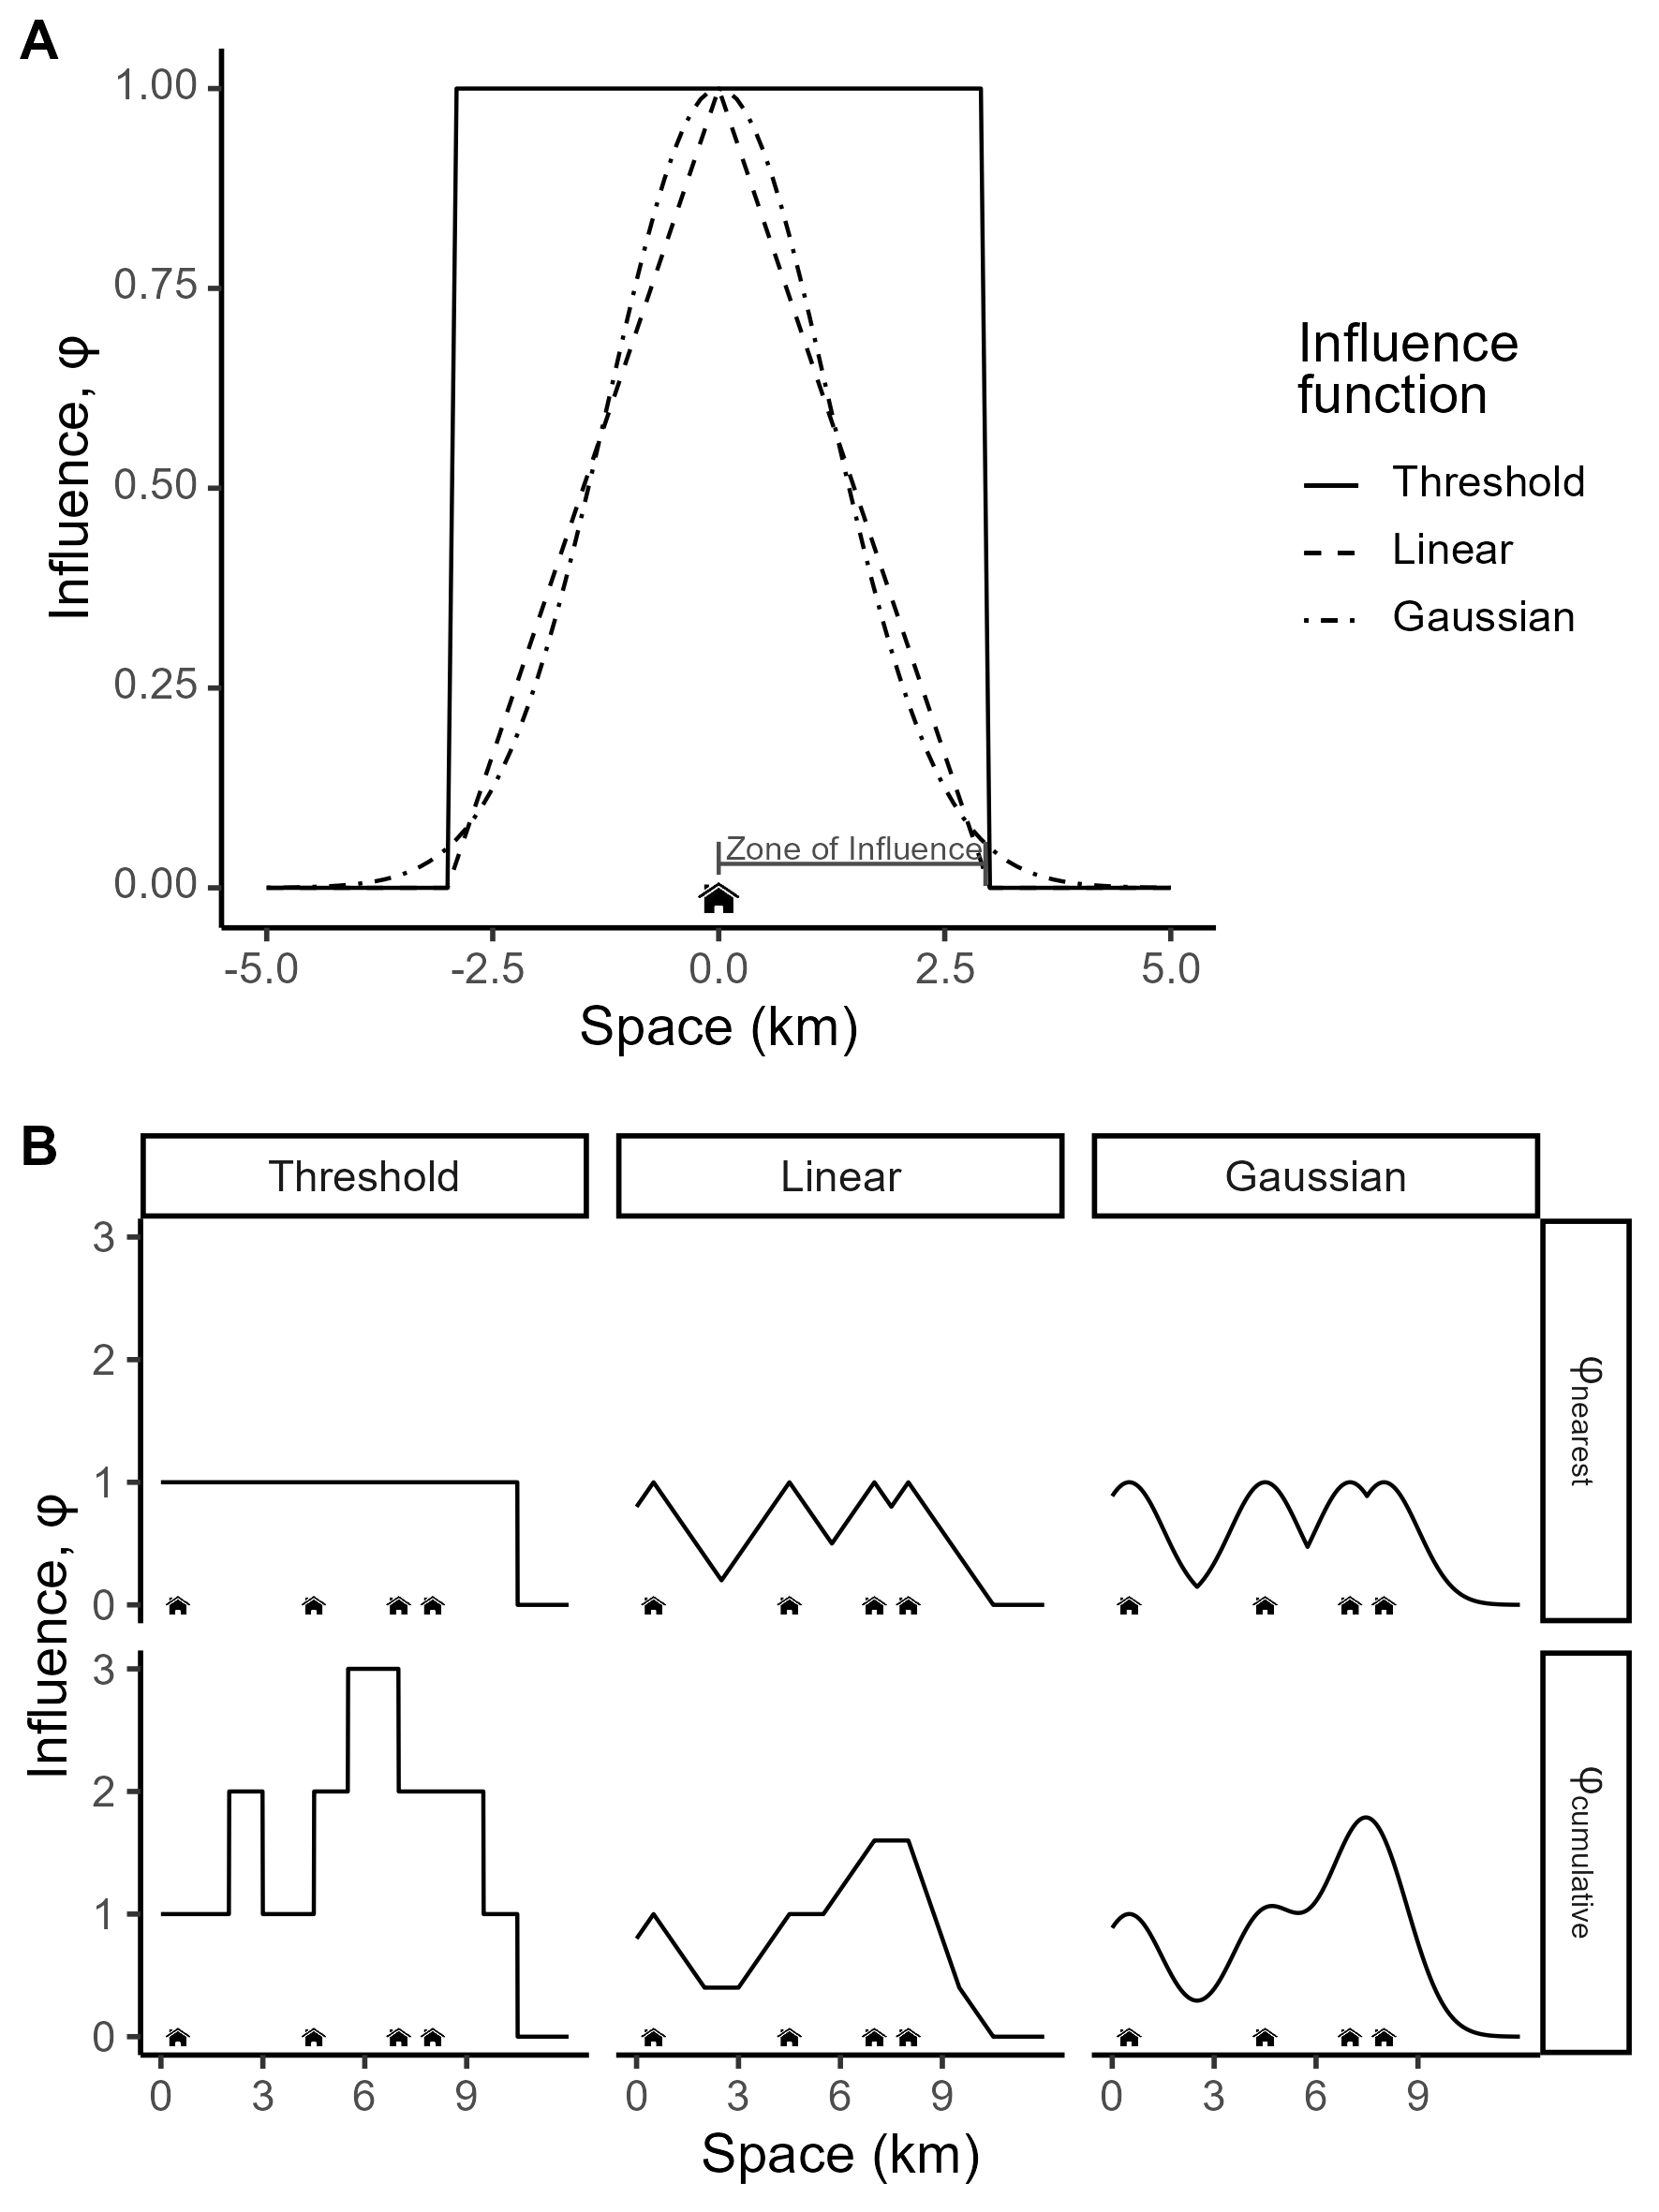
\includegraphics[width=0.9\textwidth]{figures/ZoI_conceptual.png}
\caption{\label{fig:zoi_conceptual} Illustration of the influence ($\phi_{i_k}$) of infrastructure features against the distance from those features ($d_{i_k}$), simplified for one dimension and using houses as an example. (A) Examples of influence functions according which the influence of the house might vary. A house has only an influence within its zone of influence (here $ZoI_{i_k} = 3 \text{ km}$). For the threshold function, the influence remains constant within the ZoI and drops to zero beyond it, whereas for both the linear and Gaussian functions it declines monotonically within the ZoI. 
%For functions that asymptotically approach zero, a cutoff must be selected to characterize the ZoI (here the ZoI is the distance where the influence decreases to $\phi_{i_k} < 0.05$). 
(B) Representation of the influence of multiple houses by considering only the nearest feature (upper row) or the cumulative influence of multiple features (bottom row), for different influence functions. If only the nearest house is considered, the influence does not exceed one; when all houses act cumulatively, their cumulative influence can be much higher than one.}
\end{figure}

To translate those representations into a mathematical form, now we decompose each of the linear terms (i.e. A, B, C, ...), in equation \ref{eqn:HSF}. Suppose that in the landscape there are $n_k$ features of the same type of infrastructure $k$, and let the influence of the feature $i$ of an infrastructure \textit{k} follow an influence function \citep[or ``weighting function", ][]{miguet_how_2017} $\phi_{i_k} = f(d_{i_k}; ZoI_k)$, where $d_{i_k}$ is the distance to a feature ($i_k$) of infrastructure type $k$ and $ZoI_k$ is its zone of influence. Figure \ref{fig:zoi_conceptual}A shows a few possible shapes for the function $\phi_{i_k}$. We can sum the effect of each feature on animal space use, so that the linear terms in equation \ref{eqn:HSF} becomes:

\begin{equation}
\label{eqn:HSFterm}
    \beta_k X_k = \sum_{i=1}^{n_k} \beta_{i_k} \phi_{i_k}
\end{equation}

Typically, only the nearest feature is considered, resulting on the implicit assumption that $\beta_i = 0$ for all $i > 1$ (where the features are ordered by increasing distance). Thus, eq. \ref{eqn:HSFterm} turns into:

\begin{equation}
\label{eqn:HSFnearest}
\begin{split}
    \beta_k X_k & = \beta_{1_k} \phi_{1_k} \\
                & = \beta_{1_k} \phi_{nearest_k}
\end{split}                
\end{equation}

where $\phi_{nearest_k}$ is the influence of the nearest feature ($i = 1$) of the infrastructure type $k$ (see Fig. \ref{fig:zoi_conceptual}B). However, possibly a more reasonable assumption would be that $\beta_{i_k} = \beta_{{(i+1)}_k} = \beta_{{(i+2)}_k} = ... = \beta_k$, i.e. that all features of a given type present the same influence around them and all $\beta$'s are identical. Thus, eq. \ref{eqn:HSFterm} is reduced to:

\begin{equation}
\label{eqn:HSFcuminf}
\begin{split}
    \beta_k X_k & = \beta_k \sum_{i=1}^{n_k} \phi_{i_k} \\
                & = \beta_k \phi_{cum_k}
\end{split}
\end{equation}

where $\phi_{cum_k} = \sum_{i=1}^{n_k} \phi_{i_k}$ is the cumulative influence measure and is proportional to 
%what has been called 
the ``density" of features in space \citep[e.g.][]{panzacchi_searching_2015}. The cumulative influence measure is easily calculated using geographical information systems, e.g. through neighborhood analysis, and can be rescaled to meaningful measurement scales, such as the number of point features per km\textsuperscript{2}. For the derivation of similar equations for variables represented as lines and areas, see Appendix A.

%Analogous to \citet{lee_estimating_2020}'s recasting of the identification of the ZoI of a single (i.e. the nearest) infrastructure as a model selection rather than a parameterization problem, with this definition we can also estimate the cumulative effect size and the ZoI of features using model selection, which allows the process to be performed for different types of infrastructure. Beyond that, this formulation makes it possible to test for the presence of cumulative impacts of anthropogenic landscape changes by comparing models with either of the two influence measures (eq. \ref{eqn:HSFnearest} and \ref{eqn:HSFcuminf}), both based on the same decay function.

\section{When do the influence of the nearest feature and the cumulative influence represent similar spatial variation?}

A deeper look at the two influence measures -- nearest and cumulative -- is important to interpret them in ecological contexts and to investigate in which conditions they represent similar or different gradients of spatial variation. Their similarity depends on the spatial distribution of the infrastructure as well as its zone of influence, and might affect our ability to distinguish among their effects in real landscapes. To illustrate in which conditions they converge, we simulated $30 \times 30$ km\textsuperscript{2} landscapes with a constant number of point features (e.g. houses, cabins, turbines; $n = 100$) distributed following different spatial patterns, in a gradient of clustering, from regular and random to clustered (Fig. \ref{fig:simulated_landscapes}; Appendix B). For each landscape we calculated the two measures of influence ($\phi_{nearest}$ and $\phi_{cum}$) for a range of values of ZoI (from 0.06\% to 40\% of the landscape extent), using a linear decay function (Fig. \ref{fig:zoi_conceptual}). We then compared the resulting influence spatial patterns through Pearson correlation of the values of the two measures at the same coordinates. 

\begin{figure}[h]
\centering
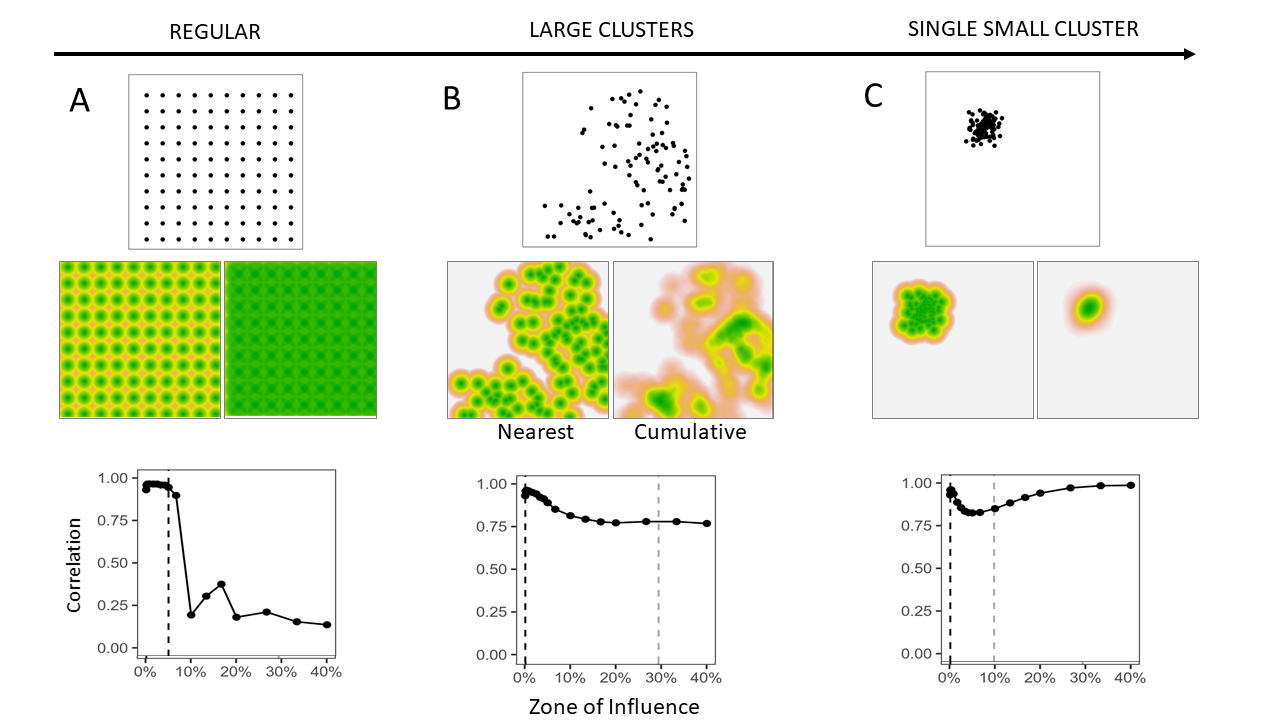
\includegraphics[width=1.3\textwidth,center]{figures/simulated_landscapes.png}
\caption{\label{fig:simulated_landscapes} Representation of the influence of nearest feature ($\phi_{nearest}$) and the cumulative influence ($\phi_{cum}$) in landscapes with point infrastructure spatially distributed in a gradient of clustering, from (A) a regular distribution 
%(e.g. a large solar power plant in a flat area) 
to (B) a set of clusters 
%(e.g. a wind industrial area formed by wind turbines built in the mountain tops) 
to (C) only one cluster. 
%(e.g. isolated village or urban center). 
The central panel shows  a visual comparison between $\phi_{nearest}$ (left) and $\phi_{cum}$ (right) when $ZoI$ is 10\% of the landscape extent. The lower panel shows the correlation between $\phi_{nearest}$ and $\phi_{nearest}$ in each landscape, as their ZoI increases. The dashed vertical lines show half the the minimum distance between features (black), beyond which there are cumulative effects of the different infrastructure, and the size of the feature clusters (grey), beyond which the correlation stops decreasing.}
\end{figure}

When $2 \cdot ZoI$ is smaller than the minimum distance between features, both measures of influence are identical (Fig. \ref{fig:simulated_landscapes}; $\text{correlation} = 1$ for all ZoI values below the black dashed vertical line). This happens because the ZoI of each feature is not large enough to overlap to each other -- when either the ZoI is small enough or  there is a small number of features sparsely distributed in space (Fig. 2A). As the ZoI increases, the effect of nearby features starts to accumulate and the two measures of influence begin to represent different patterns of spatial variation. This is valid for scenarios with random, regular, and slightly clustered distributions of infrastructure features (Fig. \ref{fig:simulated_landscapes}A,B, Figs. B5 and B8). In contrast, as the distribution of features gets more clumped and distributed in smaller clusters (up to a limit with a single small cluster, Fig. \ref{fig:simulated_landscapes}C), the correlation between the influence measures goes through a point of inflection as the ZoI increases, beyond which it increases with ZoI (Fig. B5D-F). The point where the correlation between the influence measures stop decreasing is defined by the size of the clusters (grey dashed vertical line in Figs. \ref{fig:simulated_landscapes}B,C). For ZoI values larger than the cluster size, the two influence measures start to converge again. This happens because, while the variation in cumulative influence increases continuously with ZoI, the variation in the influence of the nearest feature tends to get stable for large enough ZoI values (Figs. B5 and B7). That is the point beyond which it might get harder to distinguish between the effect of each feature alone, regardless of the influence measure, and the effect of a collection of features transforms into that of a ``super-feature" (e.g. groups of houses or wind turbines behave as urban areas or wind parks, respectively). 
%Overall, the correlation between the influence measures is high (Fig. \ref{fig:simulated_landscapes}). 
When the correlation between influence measures is higher, it might be difficult to distinguish whether the impacts of a given infrastructure type accumulate or not. 
%However, in other cases (such as the correlation inflection point mentioned above) it might be easier to detect differences and test for cumulative effects.
However, whether a given biological response variable is affected by only the nearest feature or the cumulative influence of multiple features (or none) remain an empirical question to be explored in real landscapes. 

\section{Empirical demonstration: cumulative influence of infrastructure on reindeer space use}

\subsection{Study area, ecological data, and methods}

In our empirical demonstration we aimed to assess if and how the impacts of multiple infrastructure affect mountain reindeer space use during summer in Southern Norway. Reindeer are highly sensible to human activity, and the wild populations in Norway are the last remaining ones of this species in Europe. We used GPS tracking data from the Hardangervidda reindeer population, the largest population of wild mountain reindeer (Fig. \ref{fig:prediction_maps}). During summer, the area is mostly used for tourism. It has 14,154 private cottages, 26 large tourist cabins, and hundreds of kilometers of trails, besides roads and small tourist cabins (Fig. C2). We used data from 48 (??) female reindeer collected between 2001 and 2010 \citep[see][for further details]{panzacchi_searching_2015} and selected July as a month representative of the summer. To assess reindeer habitat selection using a use-availability setup, each used GPS point was compared against 9 available locations created at random within the area occupied by the population (Fig. \ref{fig:prediction_maps}) and annotated with environmental covariates.

To account for bio-climatic-geographical variation in environmental characteristics we used the four first components from a large principal component (PC) analysis conducted for Norway \citep{bakkestuen_step-less_2008}, which correspond to gradients of (1) PC1 - continentality, (2) PC2 - altitude, (3) PC3 - terrain ruggedness, and (4) PC4 - solar radiation. We included a quadratic term for PC1 and PC2 to account for niche ``optima" \citep[\textit{sensu}][]{panzacchi_searching_2015}. We also used a satellite-based land cover map with 25 vegetation classes, which we further grouped (see Table C2). Because of correlations among covariates, and to keep model fitting relatively simple, we estimated the cumulative impacts for two anthropogenic variables: private cottages and large tourist cabins.

For each infrastructure type we calculated the influence measures for 8 different ZoI, from 100 to 20,000 m. For each ZoI, we used four influence functions, to account for different shapes of the variation of the infrastructure influence within the ZoI (Fig.~\ref{fig:zoi_conceptual}A): threshold, linear decay, Gaussian decay, and exponential decay, and made two assumptions for the impact of additional features, leading to the measures of influence from the nearest feature ($\phi_{nearest}$, eq. \ref{eqn:HSFnearest}) and cumulative influence ($\phi_{cum}$, eq. \ref{eqn:HSFcuminf}; see Fig.~\ref{fig:zoi_conceptual}B). We then fitted HSFs (eq. \ref{eqn:HSF}) combining the effects of infrastructure, land cover, and bio-climatic data through binomial generalized linear models \citep{fieberg_how_2021}. 

Model fitting consisted in two steps. We first fitted single-infrastructure models in a procedure of variable selection \citep{burnham_model_2002} to assess the most likely influence functions and ZoI for each infrastructure type, while checking for the correlation between covariates. Single-infrastructure HSF were fitted using the \verb|multifit| function in R \citep{huais_multifit_2018} and compared using AIC. Second, using the most likely influence functions and ZoI from the single-infrastructure models, we fitted multi-infrastructure HSF to assess the combined impacts of multiple types of infrastructure, in an approach similar to \citet{laforge_process-focussed_2015}. 

To quantify the impacts of infrastructure, we used eq. \ref{eqn:HSFterm} and multiplied the magnitude of the impacts -- the coefficients of the fitted model -- by the influence measures included the model. We then estimated habitat suitability by predicting the HSF (eq. \ref{eqn:HSF}) over the space and rescaling the predicted values to the interval [0, 1]. For more details on the data, environmental covariates, modeling, and results, see the Appendix C.

\subsection{Cumulative impacts on reindeer space use}

We found strong evidence that the impacts of private cottages and tourist cabins accumulate over reindeer habitat selection, leading them to avoid being close to these infrastructures (Table C2). While private cottages exerted a constant cumulative influence within a ZoI of 10 km, large tourist cabins followed an exponentially decaying cumulative influence in a ZoI of 20 km (Fig. \ref{fig:impact_plot}; Table C2). Notice that, as parameterized here, for the tourist cabins an exponential decay with ZoI of 20 km means
that the influence of cabins decrease to half of its maximum value
at ca. 5 km from the infrastructure (Fig. \ref{fig:impact_plot}). As a comparison, the most plausible model with a covariate for the influence of the nearest feature was ranked 26\textsuperscript{th} in the model selection ($\Delta AIC = 921$), and the most likely model including the log-distance to the nearest feature was ranked 44\textsuperscript{th} ($\Delta AIC = 1197$, Table C2).

\begin{figure}[h]
\centering
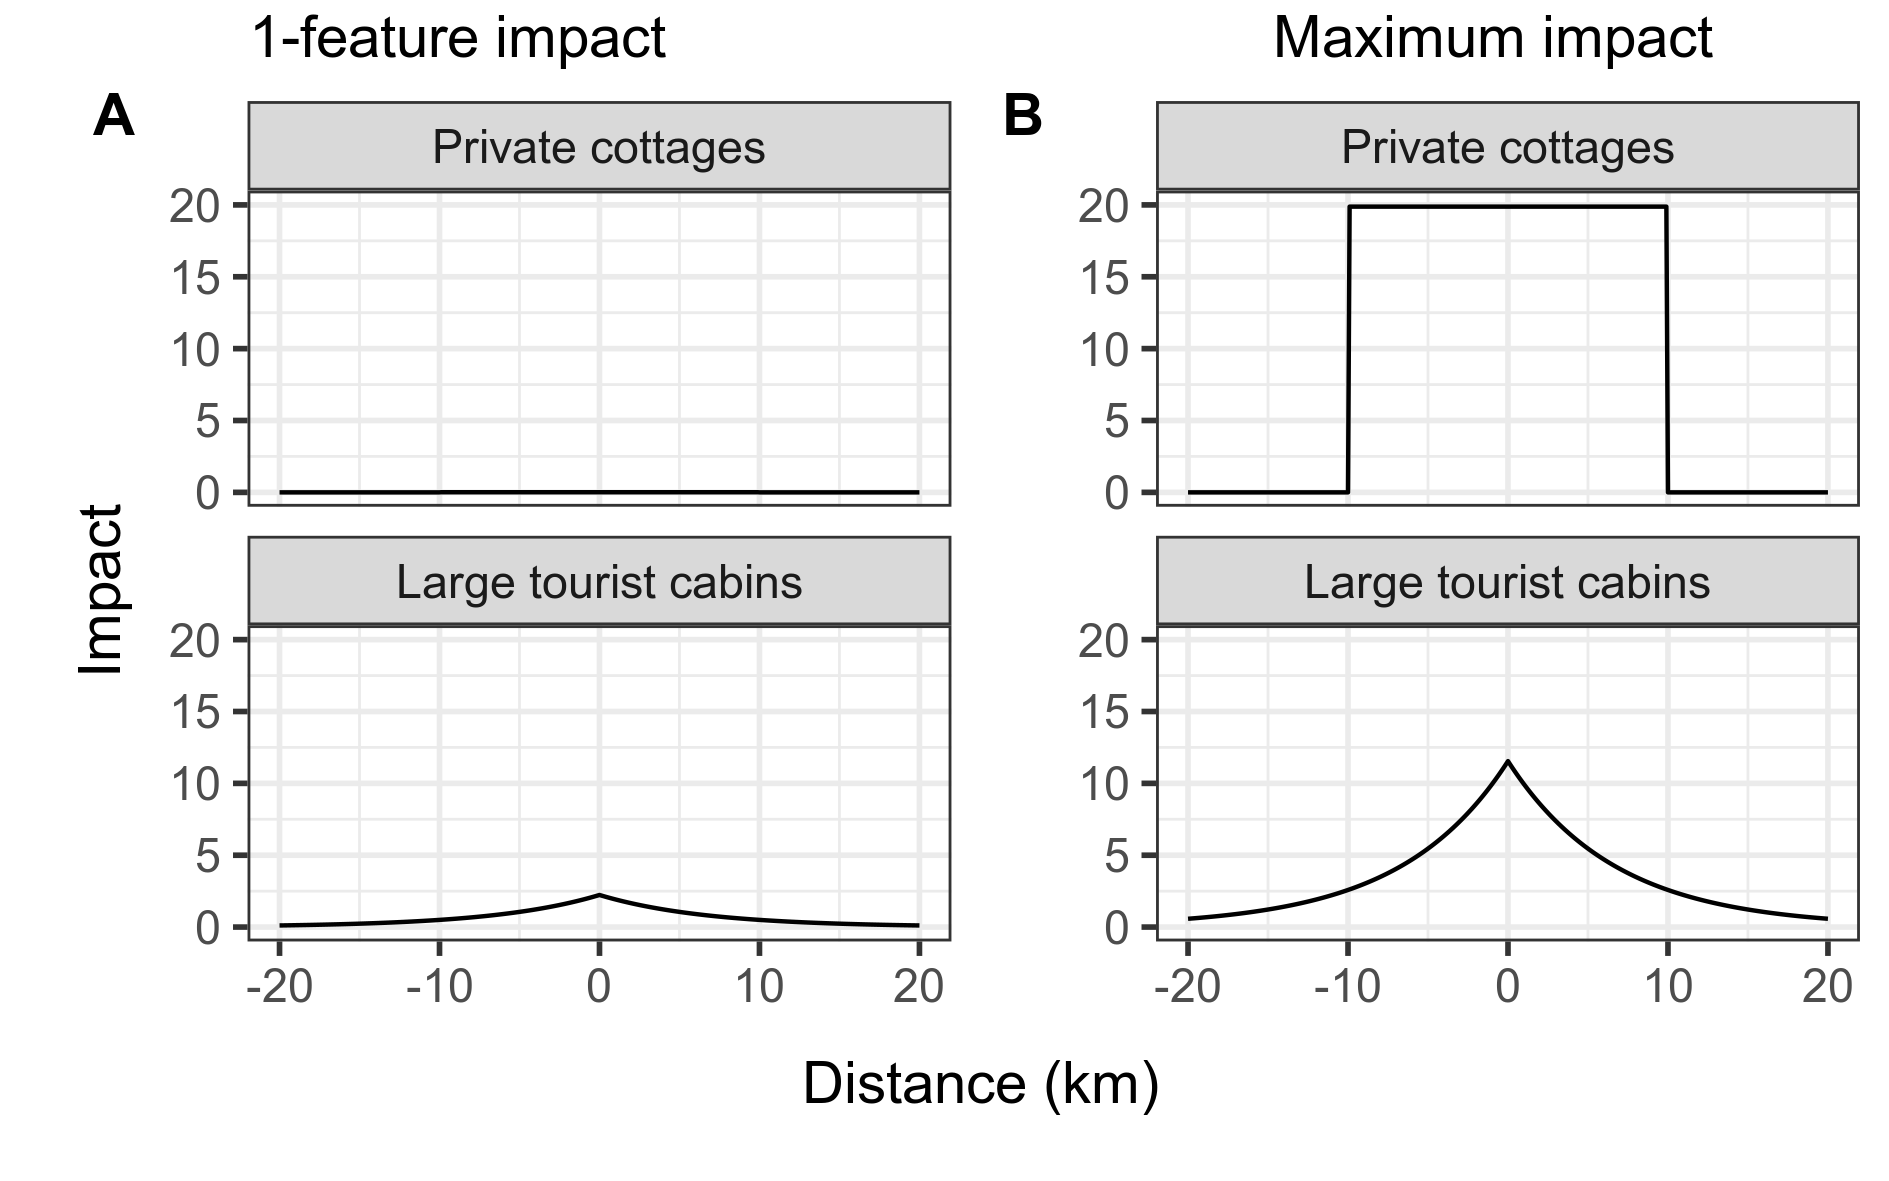
\includegraphics[width=1\textwidth,center]{figures/reindeer_zoi_impact_single_multiple_features.png}
\caption{\label{fig:impact_plot} Impact of private cottages and public cabins considering (A) only 1 feature and (B) the maximum number of features of each type of infrastructure in the study area (2664 for cottages, 5 for cabins). The impact is the multiplication between the magnitude of the impact (model coefficients) and the cumulative influence function ($\phi_{cum}$). While the impact of only one private cottage is negligible, at their maximum densities the cumulative impact of private cottages is higher than that of tourist cabins.}
\end{figure}

The estimated magnitude of the impact of a single private
cottage ($\beta_{cottage} = -0.0081$) was much smaller than that of a single tourist cabin
($\beta_{\text{private cabin}} = -2.654$; Fig. \ref{fig:impact_plot}A, Table C3), which is reasonable since the former are used by much less people than the latter. However, since
private cottages occur at higher densities, in some areas their overall impact 
is larger than that of tourist cabins. If we take the areas with the 
higher cumulative influence of infrastructure in Hardangervidda -- where the number of private cottages sum to 2664 
and the (exponentially weighted) number of tourist cabins sum to 5 -- the impact of 
private cottages agglomerates is nearly twice that of tourist cabins
 (Fig. \ref{fig:impact_plot}B and 4). Following the HSF coefficient interpretation from \citet{fieberg_how_2021}, considering that all other conditions are kept similar, a reindeer avoids an area 14.43 times more strongly than another area with
330 less private cottages in a radius of 10 km. That is approximately the same difference in avoidance a reindeer presents among two areas 
that differ in 1 tourist cabin in a radius of 20 km (Appendix C).

When cumulative impacts of infrastructure are predicted in space by multiplying the magnitude of the impacts to the cumulative influence measures (eq. \ref{eqn:HSFcuminf}), we see how the relative impact of private cottages and tourist cabins changes across space (Fig. \ref{fig:prediction_maps}). While the impact value for private cottage rises to ca. 20 in the areas with the highest cumulative influence of cottages, it hardly goes above 10 for tourist cabins. As a consequence of the combined impact of multiple infrastructure, and given reindeer
avoided high densities of both infrastructure types at relatively large extents, 
areas of high habitat suitability for reindeer correspond to those in which the
cumulative influence of both infrastructure is low -- what matches the
locations used by reindeer, indicated through the GPS data (Fig. \ref{fig:prediction_maps}).

\begin{figure}[h]
\centering
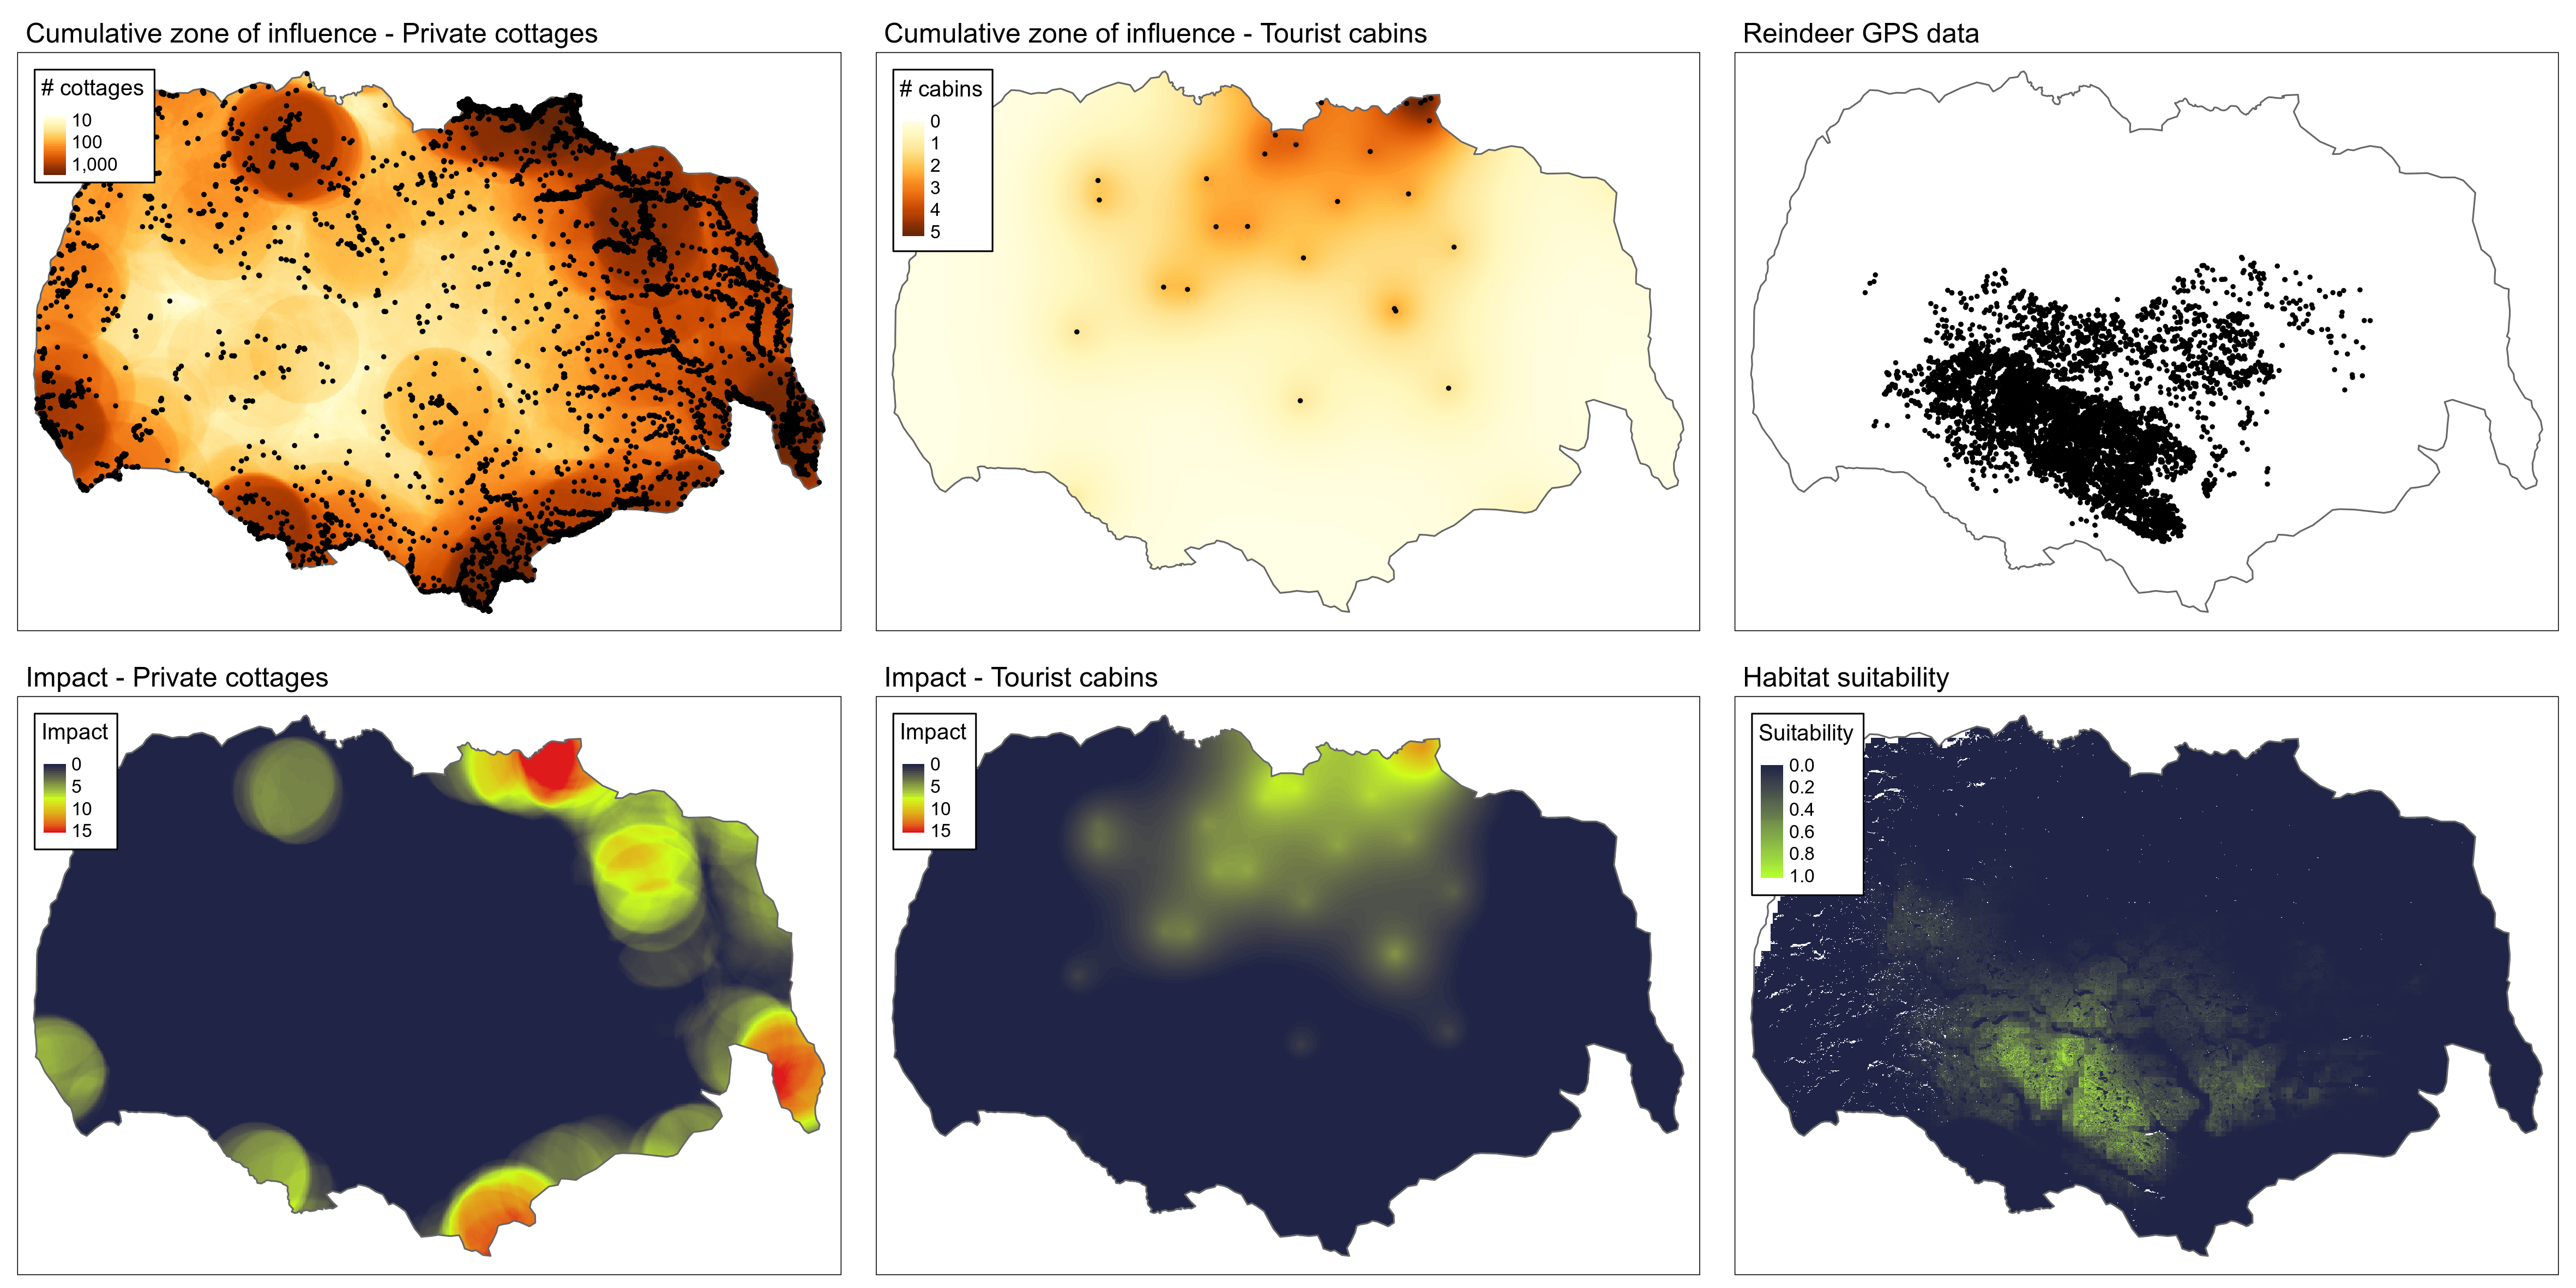
\includegraphics[width=1.3\textwidth,center]{figures/reindeer_results_prediction_maps.png}
\caption{\label{fig:prediction_maps} Maps of the most parsimonious cumulative influence variables (private cottages: threshold with 10km ZoI; tourist cabins: exponential decay with 20 km ZoI) and their estimated impacts on reindeer habitat selection. These maps are showed alongside the reindeer GPS locations in the Hardengervidda wild reindeer area and the estimated reindeer habitat suitability.}
\end{figure}

%\section{Tools to assess cumulative impacts of infrastructure}

%To ease the application of the cumulative effects assessment proposed here, we developed the \verb|oneimpact| R package. Based on raster maps with the location of infrastructure or any type of landscape variable (e.g. specific land cover or land use types), it allows the calculation of the influence from the nearest infrastructure feature ($\phi_{nearest}$ in eq. \ref{eqn:HSFnearest}) through the function \verb|calc_influence_nearest()| and the cumulative influence of multiple infrastructure ($\phi_{cum}$ in eq. \ref{eqn:HSFcuminf}) through the \verb|calc_influence_cumulative()| function. Both functions can be run using different filters or decay shapes (argument \verb|type|) -- exponential decay, linear (Bartlett or tent-shaped) decay, Gaussian (or half-normal) decay, threshold (or step) influence -- for multiple zones of influence (parameter \verb|zoi|), with the decay functions being parameterized on the ZoI. Besides those pre-defined decay functions, it also allows one to create user-defined filters (weight matrices) for cumulative effects estimation through the function \verb|create_filter()|.

%Furthermore, the \verb|oneimpact| package allows the calculation of the influence measures on both R \citep{r_core_team_r_2020} and GRASS GIS \citep{grass_development_team_geographic_2017}. On the one hand, the implementation in R allows high accessibility to users, since R is the most used statistical tool by ecologists \citep{lai_evaluating_2019}. On the other hand, the package provides a direct link from R to the powerful algorithms of GRASS GIS, so the influence measure calculation might be performed for very large and fine-scale spatio-temporal datasets. An introduction to the essential functions to calculate the two influence measures is found in Appendices D (for R) and E (for GRASS GIS). The \verb|oneimpact| package is available in the Github repository: \url{github.com/NINAnor/oneimpact}.

%\todo[inline]{Should we include a table with the functions and a short description?  Function name, description, type methods, input, output. Maybe in Appendix D.}

\section{Discussion}

There is an urge to evaluate, debate, and inform scientists, decision-makers, and the public in general about the past, current, and future effects of global infrastructure on biodiversity \citep{laurance_conservation_2018}. Most of the decisions and regulations made for infrastructure projects are performed with little knowledge about the multiple potential impacts on the ecosystems where they are built and the species living therein. Even when environmental impact assessments are well conducted, they hardly estimate the cumulative effects of those infrastructure with pre-existing ones or with other development projects planned for the same region \citep{laurance_roads_2017, johnson_regulating_2011}. In great part, this happens because current approaches and tools still lack in their ability to incorporate cumulative impacts \citep[but see][for recent advances]{gillingham_integration_2016}. Building upon previous frameworks to understand cumulative impacts \citep{naugle_unifying_2011} and by adapting concepts and tools from the landscape ecology literature into the nearest and cumulative influence measures, here we gave a step further in developing a clear way to assess cumulative effects and impacts of infrastructure on biodiversity. The approach proposed here allows one to: (i) quantify the cumulative impact of multiple infrastructure of the same type, the main focus of our approach; (ii) test whether there are cumulative impacts for each type of infrastructure, by comparing the influence of the nearest feature and the cumulative influence as predictors of biological responses, within ecological models; and (iii) estimate the zone 
%and area 
of influence for multiple types of infrastructure. 
%Here we depicted scenarios where each of the influence measures might converge or diverge, presented a case study to illustrate it, and offered tools to allow their application in ecological studies and environmental impact assessments.

\subsection{Applying the cumulative influence approach to impact assessment}

In our empirical demonstration with mountain reindeer in Norway, we found a strong support for the hypothesis of cumulative impacts of private cottages and tourist resorts on reindeer habitat selection, with large ZoI -- up to 20 km. Quantifying the impacts based on their magnitude and influence function allows us to compare the effects of different types of infrastructure. While the impact of a single cottage is smaller than that of a single tourist cabin, it can be much higher in areas where many private cottages are aggregated, because their influence accumulates over space (Fig. \ref{fig:impact_plot} and \ref{fig:prediction_maps}, Fig. C5). We also found all models based on the influence of the nearest feature to be much less supported by the data than the ones incorporating the cumulative influence of multiple features. This includes the models based on the log-distance to the nearest feature, which is a common proxy for the effect of infrastructure and landscape variables in the ecological literature \citep[e.g.][]{torres_assessing_2016,polfus_identifying_2011}. This means that, by limiting measures of infrastructure influence to the nearest feature only, researchers and practitioners have been ignoring the possibility of cumulative impacts in ecological studies and impact assessments, what limits our overall understanding of the impacts of landscape change on biodiversity.

Three points must be highlighted regarding the interpretation of the ZoI in real contexts.
First, if different influence functions are found to affect the ecological response under study, the ZoI represents distinct areas affected by infrastructure. For instance, while we found a constant influence of private cabins in a ZoI of 10 km, for tourist cabins we found an exponential decay of the influence of these infrastructure as one gets far from them, which means not all 20 km around the resorts are affected equally. Therefore, to understand how the impact of infrastructure change across space it must be assessed by combining the magnitude and the influence function that define the impact (eq. \ref{eqn:HSFterm}, Fig. \ref{fig:impact_plot} and \ref{fig:prediction_maps}). Second, as a consequence of different shapes of the influence within the ZoI, the area affected by infrastructure or landscape changes of a given type might drastically change. Indeed, in a study on bird and insect abundance, \citet{miguet_how_2017} showed that the area affected by landscape variables can increase by a factor of up to 5.7 when one uses a distance-weighted influence measure (as the exponential and Gaussian ones presented here), in comparison to a threshold-based landscape measure. 

\textbf{discuss better this point and see if we should keep it like that:} \\
Third, given that the estimation of $\beta$ and $\phi$ is independent, the most likely ZoI can differ significantly between $\phi_{nearest}$ and $\phi_{cum}$, depending on the abundance and spatial distribution of features. For private cottages, which are present at high densities in our study area, the estimated ZoI for the cumulative influence was 10 km and the magnitude of the impact was small (Fig. C3). In contrast, if only the nearest feature was considered, the estimated ZoI would be ten times lower (~1 km) and the magnitude of the impact would be several orders of magnitude higher. This was not the case for tourist cabins, however, which are scarce and sparsely distributed in the study area (Fig. C4).    

%For illustrative purposes, we used data from the wild reindeer population in Hardangervidda and included only two types of infrastructure. However, \citet{panzacchi_searching_2015} suggest that estimates of species niches and responses to infrastructure can be poor when based on single populations. For more comprehensive analyses, we suggest that habitat selection models, ecological niche models, occupancy or other ecological models using this approach to consider biological data from different populations and areas, to include as much as possible variation on landscapes and allow the estimation of cumulative functional responses in impact assessment of infrastructure over ecological processes.  

\subsection{Assumption, advantages, and limitations of the approach}

As formulated here, the influence of the nearest feature ($\phi_{nearest}$, eq. \ref{eqn:HSFnearest}) and the cumulative influence ($\phi_{cum}$, eq. \ref{eqn:HSFcuminf}) are calculated before model fitting through the \verb|oneimpact| R package or though geographical information system tools. Here lies one of the main strengths of the approach: the cumulative impacts of multiple features of an infrastructure are estimated through selection of models with either of the influence measures, for instance through model performance measures (e.g. AIC or $R^2$; \citealt{jackson_are_2015, huais_multifit_2018}), without the necessity of repeated model fitting and complex parameterization of non-linear functions \citep{lee_estimating_2020}. This allows one to estimate the influence function and the ZoI for several types of infrastructure. It also allows fitting models for large datasets \citep[millions of points, e.g.][]{tucker_moving_2018} encompassing large study areas and fine resolution landscape covariates, what makes the approach applicable over a wide range of fields in ecology. Furthermore, the pre-computation of $\phi_$ makes their visualization easy and their calculation computationally efficient and flexible.
%, allowing one to represent influence decays following different shapes \citep[e.g. threshold or exponential decay, as in ][]{miguet_how_2017}. 
% I could add something here about the discussion over model parameterization vs model selection for the definition of scales of effect, but I am not sure if it is worth it.

Our formulation of the influence functions follow two main assumptions. First, $\phi$ is assumed present a constant ZoI, regardless of the density of points in an area. A possibly more reasonable assumption would be to consider that the ZoI of a single of few features is smaller than that of a clusters of features, which are expected to cumulatively affect a wider area. Analogous calculations with variable function size have been implemented for decades in adaptive kernel density estimation [REF], so this premise can in principle be relaxed. Second, our formulation represent two extremes where only the nearest feature influence a focal ecological process ($\beta_i = 0$ for $i > 1$) or all features affect the process equally ($\beta$ is constant over all features). This is the simplest form of accounting for cumulative effects of multiple features of the same type. The advantage of this formulation lies on the independence between the magnitude of the impacts ($\beta$'s) and the influence functions ($\phi$), what makes it possible to pre-compute $\phi$ in GIS before model fitting. However, more complex formulations could be extended from eq. \ref{eqn:HSFterm}, for instance by considering that the influence of multiple features accumulate yet the closest one exerts a larger influence than features far away (higher $\beta$ for the nearest feature).

Through simulations, we showed that $\phi_{nearest}$ and $\phi_{cum}$ represent similar gradients of spatial variation when the spatial distribution of infrastructure features is sparse and the ZoI is small (so that the features are too spaced for their effects to accumulate) and when the features are clustered and ZoI is large (in which case the clusters of features act as ``super-features", e.g. urban areas instead of houses; Appendix B). In these two situations, due to their correlation, one might be limited in distinguishing whether the impacts of multiple infrastructure on biodiversity accumulate. This might be assessed prior to statistical analysis through the computation of both influence measures at multiple ZoI and a careful evaluation of their correlations. However, as the ``true" ZoI of an infrastructure type is hardly known in advance for any system, we recommend a general approach of computing and using the two influence measures, to test if there is evidence of cumulative impacts in the different ecological systems and processes.

It is important to remark that the extent of the study area and the zones of influence to be tested must be carefully selected, especially in cumulative impact assessment where the interplay between multiple factors may produce complex setups. First, the effects of infrastructure on ecological processes might differ depending of the extent of the study area \citep{vistnes_matter_2008}. \citet{skarin_human_2014} showed that, depending of the temporal and spatial range of the study, the same type of infrastructure might vary in their effect to ecological variables, from no effect to positive or negative effects. As we show here, the spatial configuration of features and the ZoI might also affect our ability to detect if the impacts of infrastructure accumulate. 
%Furthermore, the spatial pattern of features is also affected by the selection of extent of the landscape. As an example, if the biological response is measured and assessed in a study area that comprises 10 km around a wind farm, the distribution of wind turbines might look random or somehow aggregated. However, if the study area comprises a much bigger area and the biological response is expected to respond at larger extents, and the wind farm is only located in part of that, their distribution might appear very clumped. 
Second, depending on the ecological response variable, the range of ZoI tested must encompass values much higher than the range size or even the average dispersal distance of an species \citep{jackson_what_2012}. If the ZoI values are not properly defined, the ``true" ZoI at which the ecological process being measured is affected might not be selected, the resulting estimated ZoI might be wrong and mislead management and conservation policies based on that scientific inference \citep[e.g.][]{jackson_are_2015}.

\section{Conclusions}

There is an increasing need to include cumulative impacts on environmental impact assessments and ecological studies. However, even when they are present, bringing concepts and theoretical frameworks into concrete and objective analyses to estimate cumulative impacts is often challenging and left to the responsibility of either the analysts or the regulators that review impact assessments \citep{johnson_regulating_2011}. Our approach offers resources to ecologists, environmental agencies, and stakeholders dealing with impact assessment to build concrete estimates of cumulative impacts of multiple features of an infrastructure and their zone influence. 
Even though the examples given here focused on animal space use, the cumulative influence measure we presented is applicable over a wide range
of fields within ecology. Our formulation might be easily adapted to model other types of biological responses, such as population abundance \citep[e.g.][]{benitez-lopez_impacts_2010},
species richness \citep[e.g.][]{ficetola_ecological_2009} or other measures of biological diversity and ecological processes REF[e.g.], with direct application in environmental and strategic impact assessment and integrated land use planning.
      
\section*{Authors’ contributions}

BBN, BVM, and MP conceived the idea, designed the methods, and analyzed and discussed the data. BBN, BVM, MP, TT, KL, and OS provided data. BBN and BVM wrote the first draft. All authors contributed with discussions and to the final version of the manuscript.

\section*{Acknowledgements}

We thank P. Dodonov and M.H. Vancine for discussion around the implementation of the cumulative influence measures in R and NINA (or specific people) for the GPS data collection and management. Funding?

\section*{Conflicts of Interest}

The authors declare no conflicts of interest.

\section*{Data availability statement}

GPS data is archived in Movebank (www.movebank.org) and might be accessed upon request. All environmental data was retrieved from public repositories. The \verb|oneimpact| package is open and available at \url{github.com/NINAnor/oneimpact}, and all scripts used in the analyses are available in the Github repository \url{github.com/bniebuhr/cumulative_influence_paper} (to be made public upon the acceptance of the manuscript).

\section*{Supplementary Material}

Appendix A. Deriving the cumulative influence for line and polygon representations of infrastructure. \\
Appendix B. Comparing the the influence of the nearest feature with the cumulative influence of multiple features \\
Appendix C. Cumulative influence of infrastructure on reindeer space use: fitting habitat selection models \\
Appendix D. Getting started with \verb|oneimpact|. \\
Appendix E. Calculating cumulative influence in GRASS GIS using the \verb|oneimpact| package in R.

\bibliographystyle{besjournals}
\bibliography{cuminf_bib}

\end{document}
